%********************************************
% Lab 01: Introduction to Logisim-evolution
%********************************************

\chapter{Introduction To Logisim-evolution}

%********************************************

% Section: Introduction
%********************************************

\section{Purpose}

This lab introduces the \LE logic simulator, which is used for all lab exercises in this manual. 

%********************************************
% Section: Procedure
%********************************************

\section{Procedure}

\subsection{Installation}

\LE is a Java application, so a Java runtime environment will need to be installed before using the application. Many students who are taking a digital logic class already have a Java runtime on their computer and can skip this step, but those who do not will need to install the Java runtime. That process is not covered in this manual but information about installing the Java runtime environment is available at \url{http://www.oracle.com/technetwork/java/javase/downloads/index.html}. It can be confusing to know which version of Java to download but students working on the labs in this manual only need the runtime, called \textit{JRE} on the website. Students who are also in programming classes will likely already have the runtime as part of the Java Developer's Kit (JDK). It can be tricky testing the Java installation since the Chrome, Firefox, and Edge browsers will not run Java apps, but students can open a command prompt and enter \lstinline|java -version| to see what version of Java their computers are running, if any.

\LE (\url{https://github.com/reds-heig/logisim-evolution}) is available as a free download. Visit the website and about halfway down the page find a section named ``Running logisim-evolution.'' Click the ``here'' link at the end of the first sentence in that section. 

Since the \LE file is a Java application, it does not need to be installed like most software. To start \LE, double-click the \LE shortcut. That will start Java and then run the \LE application. Also, \LE will not need to be uninstalled when it is no longer needed since it is not actually installed, the \LE file can simply be deleted.

\subsection{Beginner's Tutorial}

\LE comes with a beginner's tutorial available in \textsc{Help -> Tutorial}. That tutorial only takes a few minutes and introduces students to the major components of the application. Students should complete that tutorial before starting this lab.

\subsection{Logisim-evolution Workspace}

Start \LE by double-clicking its icon. The initial \LE window will be similar to Figure \ref{fig:01-01}.

\begin{figure}[H]
	\centering
	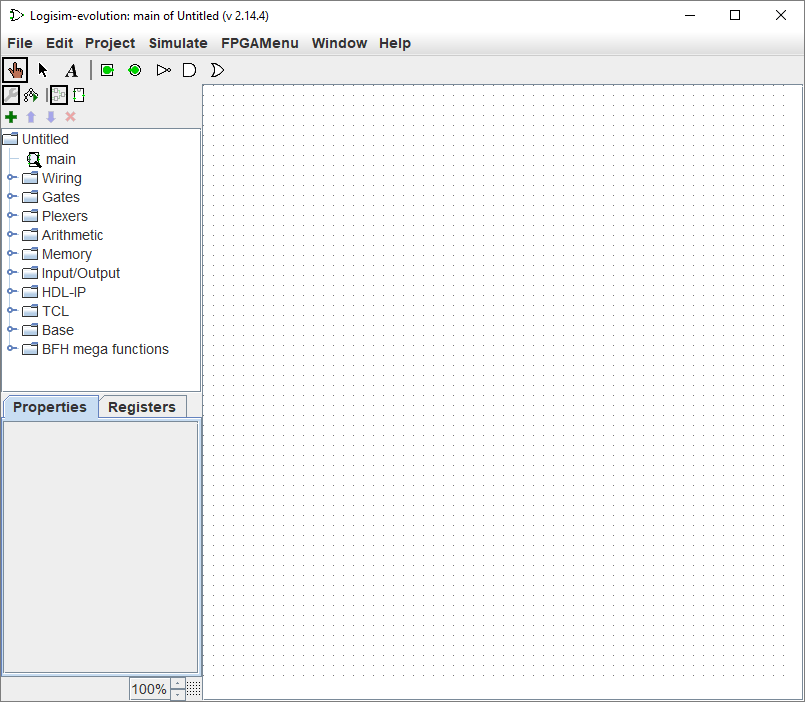
\includegraphics[width=\maxwidth{.95\linewidth}]{gfx/01-01}
	\caption{Logisim-evolution Initial Screen}
	\label{fig:01-01}
\end{figure}

The \LE space is divided into several areas. Along the top is a text menu that includes the types of selections found in most programs. For example, the ``File'' menu includes items like ``Save'' and ``Exit.'' The ``Edit'' menu includes an ``Undo'' option that is useful. In later labs, the various options under ``Project'' and ``Simulate'' will be described and used. Items in the ``FPGAMenu'' are beyond the scope of this class and will not be used. Of particular importance at this point is ``Library Reference'' in the ``Help'' menu. It contains information about every logical device available in \LE and is very useful while using those components in new circuits. 

Under the menu bar is the Toolbar, which is a row of eight buttons that are the most commonly used tools in \LE: 

\begin{itemize}
	\item \textbf{Pointing Finger}: Used to ``poke'' and change input values while the simulator is running. 
	\item \textbf{Arrow}: Used to select components or wires in order to modify, move, or delete them. 
	\item \textbf{A}: Activates the Text tool so text information can be added to the circuit. 
	\item \textbf{Green Input Port}: Creates an input port for a circuit. 
	\item \textbf{White Output Port}: Creates an output port for a circuit. 
	\item \textbf{NOT Gate}: Creates a NOT gate. 
	\item \textbf{AND Gate}: Creates an AND gate. 
	\item \textbf{OR Gate}: Creates an OR gate. 
\end{itemize}

The Explorer Pane is on the left side of the workspace and contains a folder list. The folders contain ``libraries'' of components organized in a logical manner. For example, the ``Gates'' folder contains various gates (AND, OR, XOR, etc.) that can be used in a circuit. The four icons across the top of the Explorer Pane are used for advanced operations and will be covered as they are needed. 

The Properties panel on the lower left side of the screen is where the properties for any selected component can be read and set. For example, the number of inputs for an AND gate can be set to a specific number.

The drawing canvas is the largest part of the screen. It is where circuits are constructed and simulated. 

\subsection{Simple Multiplexer}

\marginpar{Do not be concerned with the exact placement of components on the drawing canvas. They can be rearranged as the build progresses.}A multiplexer is used to select which of two or more inputs will be connected to a single output. For this lab, a simple two-input, one-bit multiplexer will be built. It is understood that students will not know the significance of a multiplexer at this point in the class, but the purpose of this lab is to use \LE to build a simple circuit and a multiplexer serves that purpose well. 

Start by clicking the \textit{And} button on the toolbar and placing two \texttt{AND} gates on the canvas. The canvas should resemble Figure \ref{fig:01-02}

\begin{figure}[H]
	\centering
	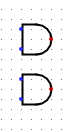
\includegraphics[width=\maxwidth{.95\linewidth}]{gfx/01-02}
	\caption{Two AND Gates}
	\label{fig:01-02}
\end{figure}

Click one of the AND gates to select it and observe the various properties available for that gate, as seen in Figure \ref{fig:01-03}. The default values do not need to be changed for this circuit; however, all circuits in this manual use the ``Narrow'' gate size in order to make the circuit fit the screen better. The other properties will be explained as they are needed.

\begin{figure}[H]
	\centering
	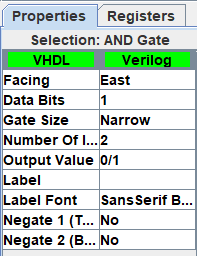
\includegraphics[width=\maxwidth{.95\linewidth}]{gfx/01-03}
	\caption{AND Gate Properties}
	\label{fig:01-03}
\end{figure}

The outputs of the two \texttt{AND} gates need to be combined with an \texttt{OR} gate. Add an \texttt{OR} gate as illustrated in Figure \ref{fig:01-04}.

\begin{figure}[H]
	\centering
	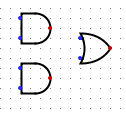
\includegraphics[width=\maxwidth{.95\linewidth}]{gfx/01-04}
	\caption{OR Gate Added to Circuit}
	\label{fig:01-04}
\end{figure}

The top input for the first \texttt{AND} gate needs two \texttt{NOT} gates (inverters) so the two \texttt{AND} gates can function as on/off switches. This is a rather common digital logic construct and when the circuit is complete it will become clear how the switching function works.

\begin{figure}[H]
	\centering
	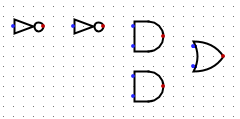
\includegraphics[width=\maxwidth{.95\linewidth}]{gfx/01-05}
	\caption{Two NOT Gates Added to Circuit}
	\label{fig:01-05}
\end{figure}

All inputs and outputs need to be added as in Figure \ref{fig:01-06}. Note: inputs are square and outputs are round. The \textit{Label} property for each input and output should be specified as in the figure. The pins are labeled according to their function in the circuit. Pin \textit{Sel} carries a signal that selects which input to connect to the output, pins \textit{In1} and \textit{In2} are the two inputs, and pin \textit{Out1} is the output. Note: output pins display a blue-colored \textsf{X} until they are actually wired to some device like the \texttt{OR} gate in the illustration.
 
\begin{figure}[H]
	\centering
	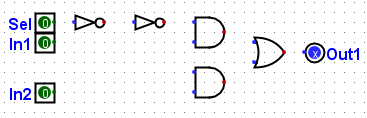
\includegraphics[width=\maxwidth{.95\linewidth}]{gfx/01-06}
	\caption{Inputs and Output Added}
	\label{fig:01-06}
\end{figure}

Finally, connect each device with a wire by clicking on the various ports and dragging a wire to the next port. To start the wire in the middle of the two NOT gates click the wire connecting those gates and drag downward. Wires will automatically ``bend'' one time but to get two bends, like between the output of an \texttt{AND} gate and the input of the \texttt{OR} gate, click-and-drag the wire from the output of the \texttt{AND} gate to a spot a short distance in front of that same gate, then release the mouse button and then immediately click again to start a new wire that will ``bend'' to the input of the \texttt{OR} gate. Only a little practice is needed to master this wiring technique.

\begin{figure}[H]
	\centering
	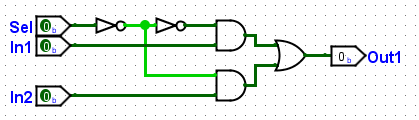
\includegraphics[width=\maxwidth{.95\linewidth}]{gfx/01-07}
	\caption{Circuit Wiring Added}
	\label{fig:01-07}
\end{figure}

To operate the circuit in a simulator, click the \textit{Pointing Finger} and ``poke'' the various inputs. If it is working properly, when the \textit{Sel} input is high then the value of \textit{In2} should be transmitted to the output, but when \textit{Sel} is low then the value of \textit{In1} should be transmitted to the output. This circuit is used to select one of two inputs to be transmitted to the output.

\subsection{Identifying Information}

Before finishing, add standard identification information near the top left corner of the circuit using the text tool (the \textit{A} button on the toolbar). That information should include the designer's name, the lab number and circuit name, and the date. Standard identification information for this lab would look like this:

\bigskip
% The minipage environment keeps the three lines together - no page break.
\begin{minipage}{\linewidth}
\begin{verbatim}
George Self
Lab 01: 2-Way, 1-Bit multiplexer
February 13, 2018
\end{verbatim}
\end{minipage}
\bigskip

\marginpar{The font properties in Figure \ref{fig:01-08} have been set to bold and a large size to make the text easier to read.}Note that \textit{Logisim-evolution} will automatically center text in a new box, so text boxes will need to be aligned after they have been created. To align the text boxes, click the \textit{Arrow} tool and use it to drag the boxes to their desired location. The completed circuit should look like Figure \ref{fig:01-08}.

\begin{figure}[H]
	\centering
	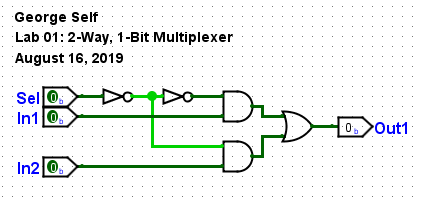
\includegraphics[width=\maxwidth{.95\linewidth}]{gfx/01-08}
	\caption{Simple multiplexer}
	\label{fig:01-08}
\end{figure}

\section{Deliverable}

The purpose of this lab is to install and test the \textit{Logisim-evolution} system and become comfortable creating a digital logic circuit. 

To receive a grade for this lab, create the Simple Multiplexer as defined in this lab, be sure the standard identifying information is at the top left of the circuit, and then save the file with this name: \textit{\texttt{Lab01\_Mux21}} (that stands for multiplexer, 2-way, 1-bit). Submit that circuit file for grading.

